%!TEX TS-program = xelatex
\documentclass[11pt]{article}

\usepackage[english]{babel}

\usepackage{amsmath,amssymb,amsfonts}
\usepackage[utf8]{inputenc}
\usepackage[T1]{fontenc}
\usepackage{stix2}
\usepackage[scaled]{helvet}
\usepackage[scaled]{inconsolata}

\usepackage{lastpage}

\usepackage{setspace}

\usepackage{ccicons}

\usepackage[hang,flushmargin]{footmisc}

\usepackage{geometry}

\setlength{\parindent}{0pt}
\setlength{\parskip}{6pt plus 2pt minus 1pt}

\usepackage{fancyhdr}
\renewcommand{\headrulewidth}{0pt}\providecommand{\tightlist}{%
  \setlength{\itemsep}{0pt}\setlength{\parskip}{0pt}}

\makeatletter
\newcounter{tableno}
\newenvironment{tablenos:no-prefix-table-caption}{
  \caption@ifcompatibility{}{
    \let\oldthetable\thetable
    \let\oldtheHtable\theHtable
    \renewcommand{\thetable}{tableno:\thetableno}
    \renewcommand{\theHtable}{tableno:\thetableno}
    \stepcounter{tableno}
    \captionsetup{labelformat=empty}
  }
}{
  \caption@ifcompatibility{}{
    \captionsetup{labelformat=default}
    \let\thetable\oldthetable
    \let\theHtable\oldtheHtable
    \addtocounter{table}{-1}
  }
}
\makeatother

\usepackage{array}
\newcommand{\PreserveBackslash}[1]{\let\temp=\\#1\let\\=\temp}
\let\PBS=\PreserveBackslash

\usepackage[breaklinks=true]{hyperref}
\hypersetup{colorlinks,%
citecolor=blue,%
filecolor=blue,%
linkcolor=blue,%
urlcolor=blue}
\usepackage{url}

\usepackage{caption}
\setcounter{secnumdepth}{0}
\usepackage{cleveref}

\usepackage{graphicx}
\makeatletter
\def\maxwidth{\ifdim\Gin@nat@width>\linewidth\linewidth
\else\Gin@nat@width\fi}
\makeatother
\let\Oldincludegraphics\includegraphics
\renewcommand{\includegraphics}[1]{\Oldincludegraphics[width=\maxwidth]{#1}}

\usepackage{longtable}
\usepackage{booktabs}

\usepackage{color}
\usepackage{fancyvrb}
\newcommand{\VerbBar}{|}
\newcommand{\VERB}{\Verb[commandchars=\\\{\}]}
\DefineVerbatimEnvironment{Highlighting}{Verbatim}{commandchars=\\\{\}}
% Add ',fontsize=\small' for more characters per line
\usepackage{framed}
\definecolor{shadecolor}{RGB}{248,248,248}
\newenvironment{Shaded}{\begin{snugshade}}{\end{snugshade}}
\newcommand{\KeywordTok}[1]{\textcolor[rgb]{0.13,0.29,0.53}{\textbf{#1}}}
\newcommand{\DataTypeTok}[1]{\textcolor[rgb]{0.13,0.29,0.53}{#1}}
\newcommand{\DecValTok}[1]{\textcolor[rgb]{0.00,0.00,0.81}{#1}}
\newcommand{\BaseNTok}[1]{\textcolor[rgb]{0.00,0.00,0.81}{#1}}
\newcommand{\FloatTok}[1]{\textcolor[rgb]{0.00,0.00,0.81}{#1}}
\newcommand{\ConstantTok}[1]{\textcolor[rgb]{0.00,0.00,0.00}{#1}}
\newcommand{\CharTok}[1]{\textcolor[rgb]{0.31,0.60,0.02}{#1}}
\newcommand{\SpecialCharTok}[1]{\textcolor[rgb]{0.00,0.00,0.00}{#1}}
\newcommand{\StringTok}[1]{\textcolor[rgb]{0.31,0.60,0.02}{#1}}
\newcommand{\VerbatimStringTok}[1]{\textcolor[rgb]{0.31,0.60,0.02}{#1}}
\newcommand{\SpecialStringTok}[1]{\textcolor[rgb]{0.31,0.60,0.02}{#1}}
\newcommand{\ImportTok}[1]{#1}
\newcommand{\CommentTok}[1]{\textcolor[rgb]{0.56,0.35,0.01}{\textit{#1}}}
\newcommand{\DocumentationTok}[1]{\textcolor[rgb]{0.56,0.35,0.01}{\textbf{\textit{#1}}}}
\newcommand{\AnnotationTok}[1]{\textcolor[rgb]{0.56,0.35,0.01}{\textbf{\textit{#1}}}}
\newcommand{\CommentVarTok}[1]{\textcolor[rgb]{0.56,0.35,0.01}{\textbf{\textit{#1}}}}
\newcommand{\OtherTok}[1]{\textcolor[rgb]{0.56,0.35,0.01}{#1}}
\newcommand{\FunctionTok}[1]{\textcolor[rgb]{0.00,0.00,0.00}{#1}}
\newcommand{\VariableTok}[1]{\textcolor[rgb]{0.00,0.00,0.00}{#1}}
\newcommand{\ControlFlowTok}[1]{\textcolor[rgb]{0.13,0.29,0.53}{\textbf{#1}}}
\newcommand{\OperatorTok}[1]{\textcolor[rgb]{0.81,0.36,0.00}{\textbf{#1}}}
\newcommand{\BuiltInTok}[1]{#1}
\newcommand{\ExtensionTok}[1]{#1}
\newcommand{\PreprocessorTok}[1]{\textcolor[rgb]{0.56,0.35,0.01}{\textit{#1}}}
\newcommand{\AttributeTok}[1]{\textcolor[rgb]{0.77,0.63,0.00}{#1}}
\newcommand{\RegionMarkerTok}[1]{#1}
\newcommand{\InformationTok}[1]{\textcolor[rgb]{0.56,0.35,0.01}{\textbf{\textit{#1}}}}
\newcommand{\WarningTok}[1]{\textcolor[rgb]{0.56,0.35,0.01}{\textbf{\textit{#1}}}}
\newcommand{\AlertTok}[1]{\textcolor[rgb]{0.94,0.16,0.16}{#1}}
\newcommand{\ErrorTok}[1]{\textcolor[rgb]{0.64,0.00,0.00}{\textbf{#1}}}
\newcommand{\NormalTok}[1]{#1}

\newlength{\cslhangindent}
\setlength{\cslhangindent}{1.5em}
\newlength{\csllabelwidth}
\setlength{\csllabelwidth}{3em}
\newenvironment{CSLReferences}[3] % #1 hanging-ident, #2 entry spacing
 {% don't indent paragraphs
  \setlength{\parindent}{0pt}
  % turn on hanging indent if param 1 is 1
  \ifodd #1 \everypar{\setlength{\hangindent}{\cslhangindent}}\ignorespaces\fi
  % set entry spacing
  \ifnum #2 > 0
  \setlength{\parskip}{#2\baselineskip}
  \fi
 }%
 {}
\usepackage{calc} % for \widthof, \maxof
\newcommand{\CSLBlock}[1]{#1\hfill\break}
\newcommand{\CSLLeftMargin}[1]{\parbox[t]{\maxof{\widthof{#1}}{\csllabelwidth}}{#1}}
\newcommand{\CSLRightInline}[1]{\parbox[t]{\linewidth}{#1}}
\newcommand{\CSLIndent}[1]{\hspace{\cslhangindent}#1}\geometry{verbose,letterpaper,tmargin=2.2cm,bmargin=2.2cm,lmargin=2.2cm,rmargin=2.2cm}

\usepackage{lineno}
\usepackage[nolists,noheads]{endfloat}
\usepackage{table}

\DeclareDelayedFloatFlavour*{longtable}{table}

\pagestyle{plain}

\tolerance=1
\emergencystretch=\maxdimen
\hyphenpenalty=10000
\hbadness=10000

\doublespacing

\fancypagestyle{normal}
{
  \fancyhf{}
  \fancyfoot[R]{\footnotesize\sffamily\thepage\ of \pageref*{LastPage}}
}
\begin{document}
\raggedright
\thispagestyle{empty}
{\Large\bfseries\sffamily Predicting metawebs: transfer of graph
embeddings can help alleviate spatial data deficiencies}
\vskip 5em

%
\href{https://orcid.org/0000-0001-6067-1349}{Tanya\,Strydom}%
%
\,\textsuperscript{1,2,‡}\quad %
\href{https://orcid.org/0000-0003-0193-5441}{Salomé\,Bouskila}%
%
\,\textsuperscript{1,‡}\quad %
\href{https://orcid.org/0000-0001-9051-0597}{Francis\,Banville}%
%
\,\textsuperscript{1,3,2}\quad %
\href{https://orcid.org/0000-0003-4036-977X}{Ceres\,Barros}%
%
\,\textsuperscript{4}\quad %
\href{https://orcid.org/0000-0002-2151-6693}{Dominique\,Caron}%
%
\,\textsuperscript{5,2}\quad %
\href{https://orcid.org/0000-0003-0452-6993}{Maxwell J\,Farrell}%
%
\,\textsuperscript{6}\quad %
\href{https://orcid.org/0000-0002-9935-1366}{Marie-Josée\,Fortin}%
%
\,\textsuperscript{6}\quad %
\href{https://orcid.org/0000-0003-3220-6161}{Victoria\,Hemming}%
%
\,\textsuperscript{7}\quad %
\href{https://orcid.org/0000-0002-4104-9463}{Benjamin\,Mercier}%
%
\,\textsuperscript{3,2}\quad %
\href{https://orcid.org/0000-0002-6004-4027}{Laura J.\,Pollock}%
%
\,\textsuperscript{5,2}\quad %
\href{https://orcid.org/0000-0001-5785-8321}{Rogini\,Runghen}%
%
\,\textsuperscript{8}\quad %
\href{https://orcid.org/0000-0002-3454-0633}{Giulio V.\,Dalla Riva}%
%
\,\textsuperscript{9}\quad %
\href{https://orcid.org/0000-0002-0735-5184}{Timothée\,Poisot}%
%
\,\textsuperscript{1,2,‡}

\textsuperscript{1}\,Département de Sciences Biologiques, Université de
Montréal, Montréal, Canada\quad \textsuperscript{2}\,Quebec Centre for
Biodiversity Science, Montréal,
Canada\quad \textsuperscript{3}\,Département de Biologie, Université de
Sherbrooke, Sherbrooke, Canada\quad \textsuperscript{4}\,Department of
Forest Resources Management, University of British Columbia, Vancouver,
B.C., Canada\quad \textsuperscript{5}\,Department of Biology, McGill
University, Montréal, Canada\quad \textsuperscript{6}\,Department of
Ecology \& Evolutionary Biology, University of Toronto, Toronto,
Canada\quad \textsuperscript{7}\,Department of Forest and Conservation
Sciences, University of British Columbia, Vancouver,
Canada\quad \textsuperscript{8}\,Centre for Integrative Ecology, School
of Biological Sciences, University of Canterbury, Canterbury, New
Zealand\quad \textsuperscript{9}\,School of Mathematics and Statistics,
University of Canterbury, Canterbury, New Zealand

\textsuperscript{‡}\,These authors contributed equally to the work\\

\textbf{Correspondance to:}\\
Timothée Poisot --- \texttt{timothee.poisot@umontreal.ca}\\

\vfill
This work is released by its authors under a CC-BY 4.0 license\hfill\ccby\\
Last revision: \emph{\today}

\clearpage
\thispagestyle{empty}

\vfill

\begin{enumerate}
    \item Metawebs, i.e.~networks of potential interactions within a
species pool, are a powerful abstraction to understand how large-scales
species interaction networks are structured.%
    \item Because metawebs are typically expressed at large spatial and
taxonomic scales, assembling them is a tedious and costly process;
predictive methods can help circumvent the limitations in data
deficiencies, by providing `draft' metawebs.%
    \item One way to improve the predictive ability is to maximize the
information used for prediction, by using graph embeddings rather than
the list of species interactions. Graph embedding is an emerging field
in machine learning that holds great potential for ecological problems.%
    \item In this perspective, we outline how the challenges associated
with inferring metawebs line-up with the advantages of graph embeddings;
furthermore, because metawebs are inherently spatial objects, we discuss
how the choice of the species pool has consequences on the reconstructed
network, but also embeds hypotheses about which human-made boundaries
are ecologically meaningful.%
\end{enumerate}


\vfill

\clearpage
\linenumbers
\pagestyle{normal}

Being able to infer \emph{potential} interactions could be the catalyst
for significant breakthroughs in our ability to start thinking about
species interaction networks over large spatial scales (Hortal et al.,
2015). Understanding species interactions holds enormous potential to
not only understand and more rapidly learn about species interactions
and metawebs, but also how changes in management of a single species may
impact non-target species. In a recent overview of the field of
ecological network prediction, Strydom, Catchen, et al. (2021)
identified two challenges of interest to the prediction of interactions
at large scales. First, there is a relative scarcity of relevant data in
most places globally -- paradoxically, this restricts our ability to
infer interactions for locations where inference is perhaps the least
required (and leaves us unable to make inference in regions without
interaction data); second, accurate predictions often demand accurate
predictors, and the lack of methods that can leverage small amount of
\emph{accurate} data is a serious impediment to our global predictive
ability. In most places, our most reliable biodiversity knowledge is
that of a species pool (\emph{i.e.} a set of potentially interacting
species in a given area): through the analysis of databases like GBIF or
IUCN, it is possible to construct a list of species in a region of
interest; but inferring the potential interactions between these species
is difficult.

Following the definition of Dunne (2006), a metaweb is the ecological
network analogue to the species pool; specifically, it inventories all
\emph{potential} interactions between species for a spatially delimited
area (and so captures the \(\gamma\) diversity of interactions). The
metaweb is not a prediction of the network at a specific point within
the spatial area it covers: it will have a different structure, notably
by having a larger connectance (see \emph{e.g.} Wood et al., 2015) and
complexity (see \emph{e.g.} Galiana et al., 2022), from any of these
local networks. These local networks (which capture the \(\alpha\)
diversity of interactions) are a subset of the metaweb's species and
their interactions, and have been called ``metaweb realizations''
(Poisot et al., 2015). Differences between local networks and their
metawebs are due to chance, species abundance and co-occurrence, local
environmental conditions, and local distribution of functional traits,
among others. Yet, recent results by Saravia et al. (2021) strongly
suggest that the local realizations only respond weakly to local
conditions: instead, they reflect constraints inherited by the structure
of their metaweb. This establishes the metaweb structure as the core
goal of predictive network ecology, as it is a required information to
accurately produce downscaled, local predictions.

Because the metaweb represents the joint effect of functional,
phylogenetic, and macroecological processes (Morales-Castilla et al.,
2015), it holds valuable ecological information. Specifically, it is the
``upper bounds'' on what the composition of the local networks, given
the local species pool, can be (see \emph{e.g.} McLeod et al., 2021);
this information can help evaluate the ability of ecological assemblages
to withstand the effects of, for example, climate change (Fricke et al.,
2022). These local networks may be reconstructed given an appropriate
knowledge of local species composition and provide information on the
structure of food webs at finer spatial scales. This has been done for
example for tree-galler-parasitoid systems (Gravel et al., 2018), fish
trophic interactions (Albouy et al., 2019), tetrapod trophic
interactions (Braga et al., 2019; O'Connor et al., 2020), and crop-pest
networks (Grünig et al., 2020). In this contribution, we highlight the
power in viewing (and constructing) metawebs as \emph{probabilistic}
objects in the context of rare interactions, discuss how a family of
machine learning tools (graph embeddings and transfer learning) can be
used to overcome data limitations to metaweb inference, and highlight
how the use of metawebs introduces important questions for the field of
network ecology.

\hypertarget{the-metaweb-is-an-inherently-probabilistic-object}{%
\section{The metaweb is an inherently probabilistic
object}\label{the-metaweb-is-an-inherently-probabilistic-object}}

Treating interactions probabilistic (as opposed to binary) is a more
nuanced and realistic way to represent interactions. Dallas et al.
(2017) suggested that most links in ecological networks are cryptic,
\emph{i.e.} uncommon or hard to observe. This argument echoes Jordano
(2016): sampling ecological interactions is difficult because it
requires first the joint observation of two species, and then the
observation of their interaction. In addition, it is generally expected
that weak or rare links to be more prevalent in networks than common or
rare links (Csermely, 2004), compared to strong, persistent links; this
is notably the case in food chains, wherein many weaker links are key to
the stability of a system (Neutel et al., 2002). In the light of these
observations, we expect to see an over-representation of low-probability
interactions under a model that accurately predicts interaction
probabilities. Yet the original metaweb definition, and indeed most past
uses of metawebs, was based on the presence/absence of interactions.
Moving towards \emph{probabilistic} metawebs, by representing
interactions as Bernoulli events (see \emph{e.g.} Poisot et al., 2016),
offers the opportunity to weigh these rare interactions appropriately.
The inherent plasticity of interactions is important to capture: there
have been documented instances of food webs undergoing rapid
collapse/recovery cycles over short periods of time (\emph{e.g.}
Pedersen et al., 2017). These considerations emphasize why metaweb
predictions should focus on quantitative (preferentially probabilistic)
predictions; this should constrain the suite of appropriate models.

Yet it is important to recall that a metaweb is intended as a catalogue
of all potential interactions, which is then filtered (Morales-Castilla
et al., 2015). In a sense, that most ecological interactions are elusive
can call for a slightly different approach to sampling: once the common
interactions are documented, the effort required in documenting each
rare interaction will increase exponentially. Recent proposals suggest
that machine learning algorithms, in these situations, can act as data
generators (Hoffmann et al., 2019): high quality observational data can
generate the core rules underpinning the network structure, and be
supplemented with synthetic data coming from predictive models,
increasing the volume of information available for inference. Indeed,
Strydom, Catchen, et al. (2021) suggested that knowing the metaweb may
render the prediction of local networks easier, because it fixes an
``upper bound'' on which interactions can exist. In this context a
probabilistic metaweb represents an aggregation of informative priors on
the interactions, elusive information with the potential to boost our
predictive ability (Bartomeus et al., 2016).

\begin{figure}
\hypertarget{fig:embedding}{%
\centering
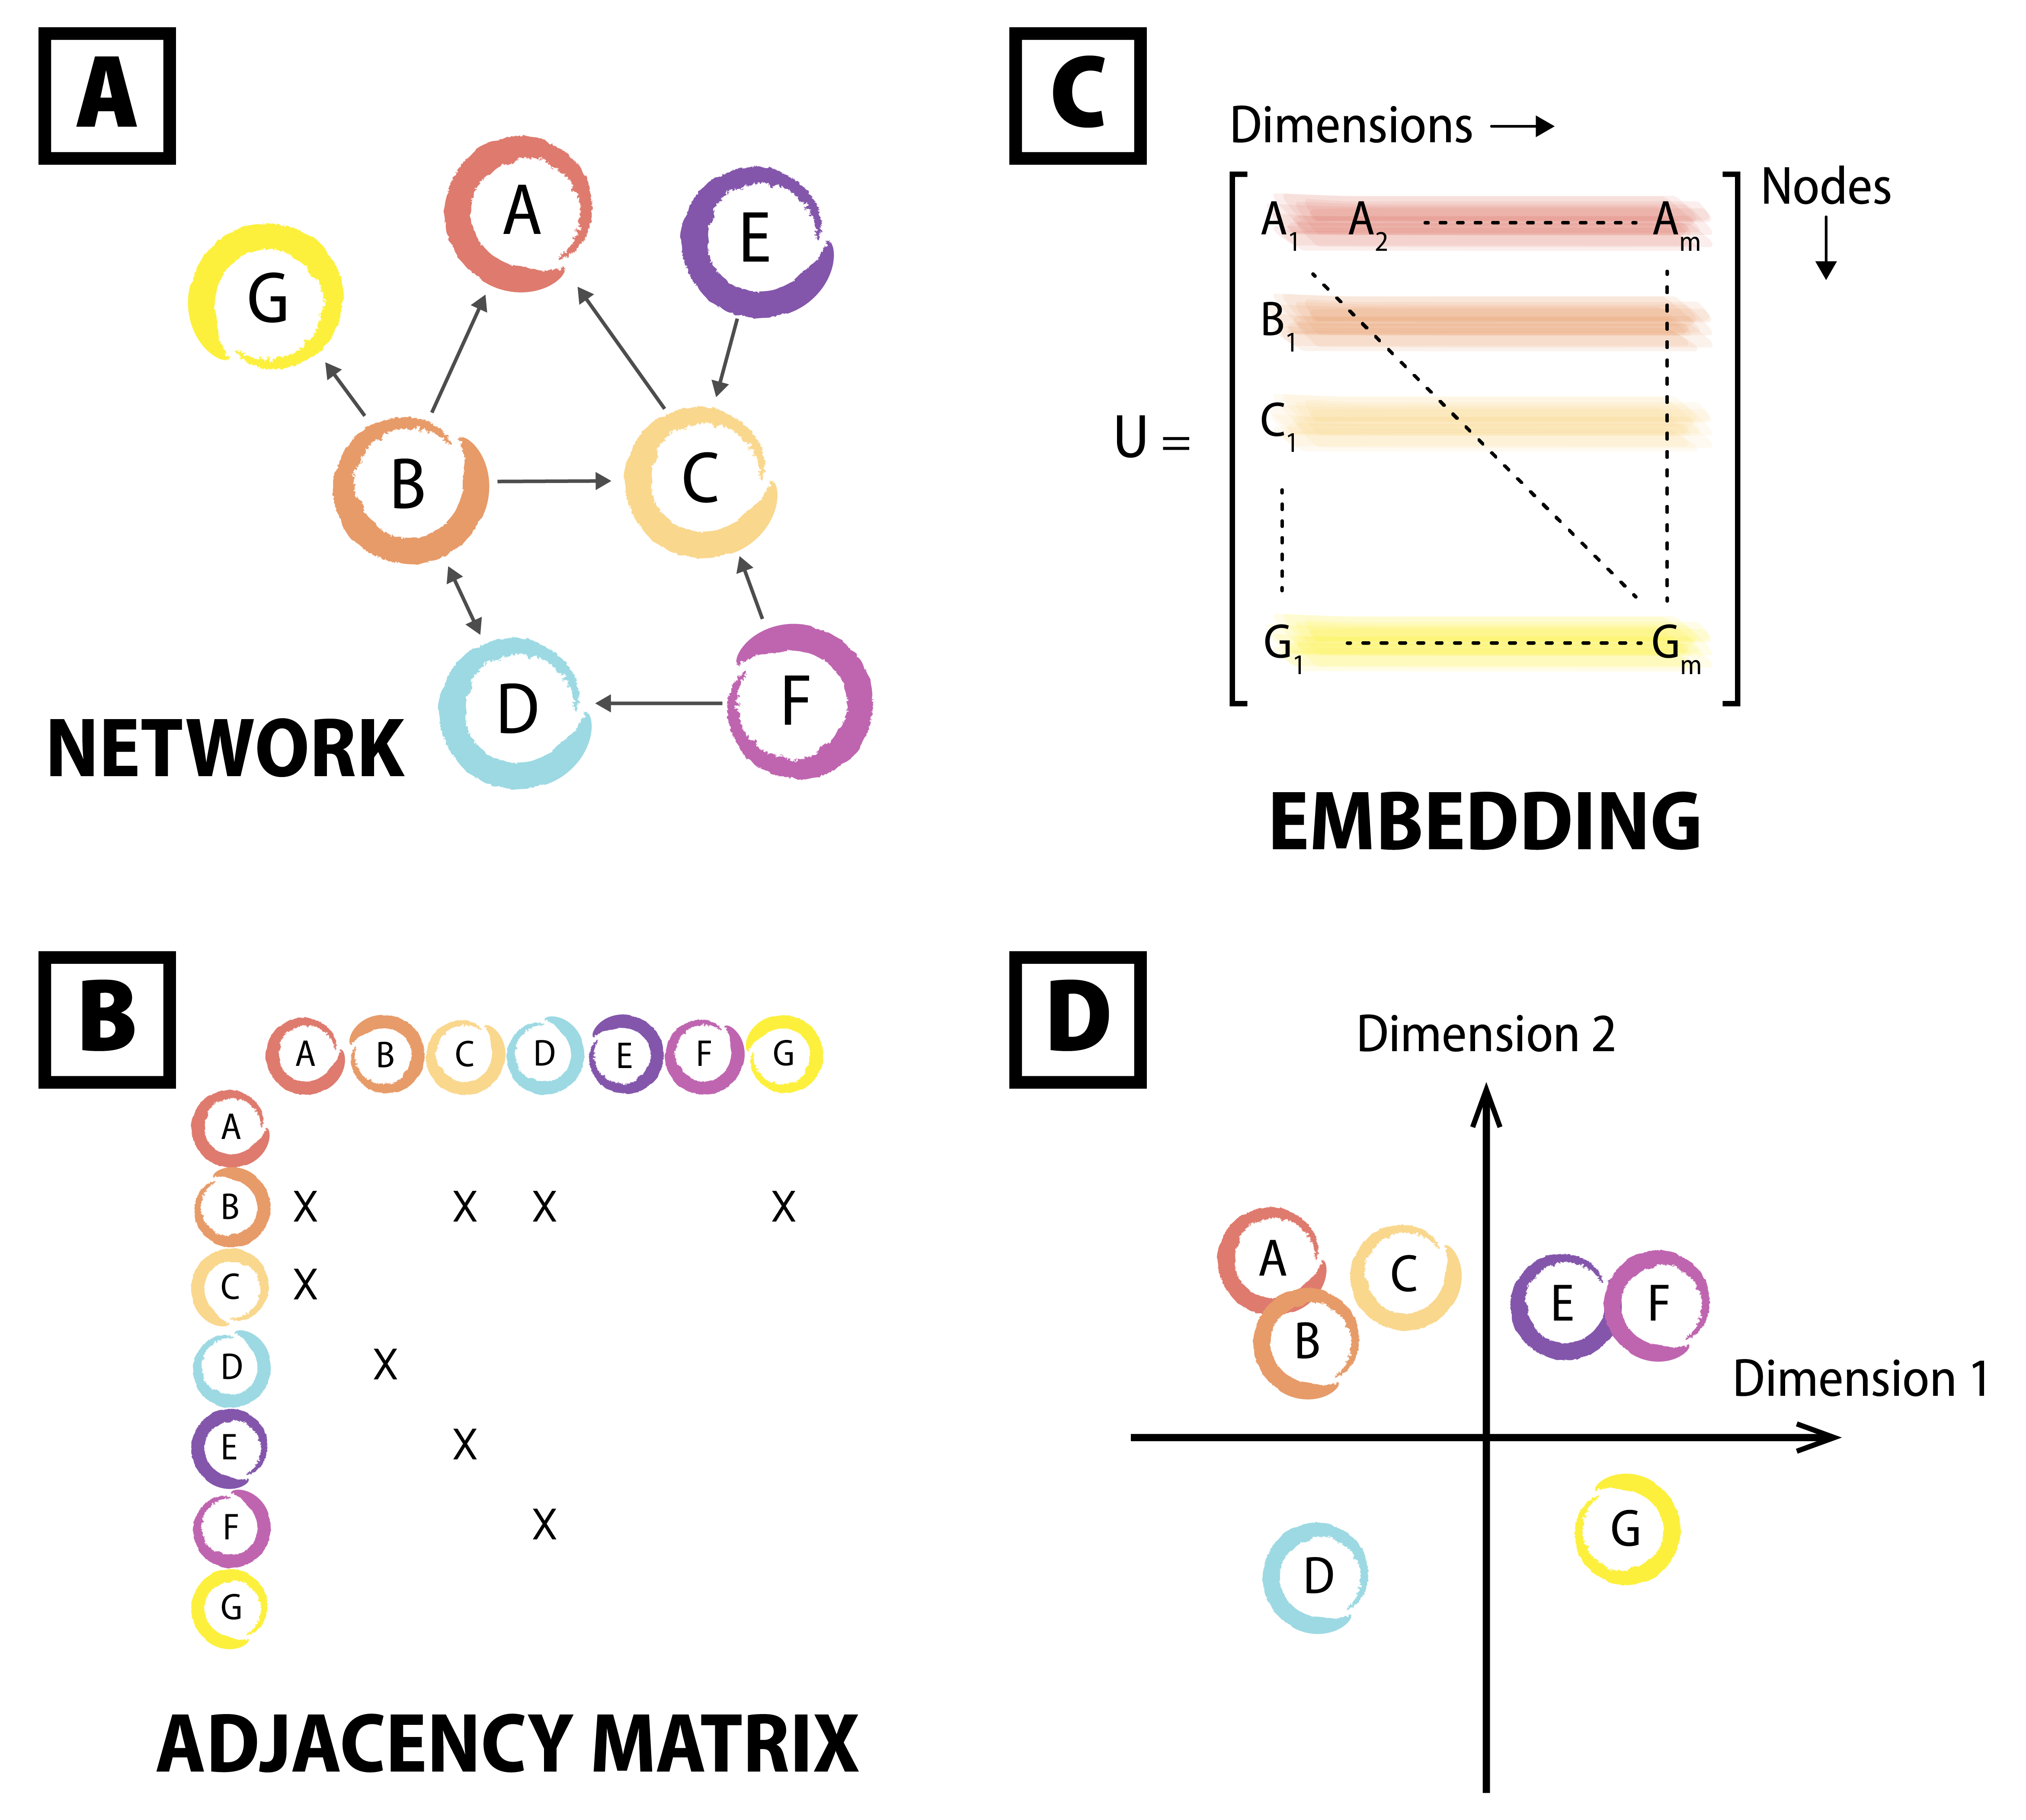
\includegraphics{figures/conceptual_embedding.png}
\caption{Overview of the embedding process. A network (\emph{A}),
represented as its adjacency matrix (\emph{B}), is converted into a
lower-dimensional object (\emph{C}) where nodes, subgraphs, or edges
have specific values (see tbl.~\ref{tbl:methods}). For the purposes of
prediction, this low-dimensional object encodes feature vectors for
\emph{e.g.} the nodes. Embedding also allows to visualize the structure
in the data differently (\emph{D}), much like with a principal component
analysis.}\label{fig:embedding}
}
\end{figure}

\hypertarget{graph-embedding-offers-promises-for-the-inference-of-potential-interactions}{%
\section{Graph embedding offers promises for the inference of potential
interactions}\label{graph-embedding-offers-promises-for-the-inference-of-potential-interactions}}

Graph embedding (fig.~\ref{fig:embedding}) is a varied family of machine
learning techniques aiming to transform nodes and edges into a vector
space (Arsov \& Mirceva, 2019), usually of a lower dimension, whilst
maximally retaining key properties of the graph (Yan et al., 2005).
Ecological networks are an interesting candidate for the widespread
application of embeddings, as they tend to possess a shared structural
backbone (Bramon Mora et al., 2018), which hints at structural
invariants that can be revealed at lower dimensions. Indeed, food webs
are inherently low-dimensional objects, and can be adequately
represented with less than ten dimensions (Braga et al., 2019; Eklöf et
al., 2013). Simulation results by Botella et al. (2022) suggest that
there is no best method to identify architectural similarities between
networks, and that multiple approaches need to be tested and compared to
the network descriptor of interest. This matches previous, more general
results on graph embedding, which suggest that the choice of embedding
algorithm matters for the results (Goyal \& Ferrara, 2018). In
tbl.~\ref{tbl:methods}, we present a selection of common graph embedding
methods, alongside examples of their use to predict species
interactions.

\hypertarget{tbl:methods}{}
\begin{longtable}[]{@{}llrr@{}}
\caption{\label{tbl:methods}Overview of some common graph embedding
approaches, by time of publication, alongside examples of their use in
the prediction of species interactions. These methods have not yet been
routinely used to predict species interactions; most examples that we
identified were either statistical associations, or analogues to joint
species distribution models. \(^a\): statistical interactions; \(^b\):
joint-SDM-like approach.}\tabularnewline
\toprule
\begin{minipage}[b]{0.11\columnwidth}\raggedright
Method\strut
\end{minipage} & \begin{minipage}[b]{0.30\columnwidth}\raggedright
Embedding approach\strut
\end{minipage} & \begin{minipage}[b]{0.16\columnwidth}\raggedleft
Reference\strut
\end{minipage} & \begin{minipage}[b]{0.32\columnwidth}\raggedleft
Application in species interactions\strut
\end{minipage}\tabularnewline
\midrule
\endfirsthead
\toprule
\begin{minipage}[b]{0.11\columnwidth}\raggedright
Method\strut
\end{minipage} & \begin{minipage}[b]{0.30\columnwidth}\raggedright
Embedding approach\strut
\end{minipage} & \begin{minipage}[b]{0.16\columnwidth}\raggedleft
Reference\strut
\end{minipage} & \begin{minipage}[b]{0.32\columnwidth}\raggedleft
Application in species interactions\strut
\end{minipage}\tabularnewline
\midrule
\endhead
\begin{minipage}[t]{0.11\columnwidth}\raggedright
tSNE\strut
\end{minipage} & \begin{minipage}[t]{0.30\columnwidth}\raggedright
nodes through statistical divergence\strut
\end{minipage} & \begin{minipage}[t]{0.16\columnwidth}\raggedleft
Hinton \& Roweis (2002)\strut
\end{minipage} & \begin{minipage}[t]{0.32\columnwidth}\raggedleft
Cieslak et al. (2020) \(^a\)\strut
\end{minipage}\tabularnewline
\begin{minipage}[t]{0.11\columnwidth}\raggedright
RDPG\strut
\end{minipage} & \begin{minipage}[t]{0.30\columnwidth}\raggedright
graph through SVD\strut
\end{minipage} & \begin{minipage}[t]{0.16\columnwidth}\raggedleft
Young \& Scheinerman (2007)\strut
\end{minipage} & \begin{minipage}[t]{0.32\columnwidth}\raggedleft
Poisot et al. (2021); Dalla Riva \& Stouffer (2016)\strut
\end{minipage}\tabularnewline
\begin{minipage}[t]{0.11\columnwidth}\raggedright
DeepWalk\strut
\end{minipage} & \begin{minipage}[t]{0.30\columnwidth}\raggedright
graph walk\strut
\end{minipage} & \begin{minipage}[t]{0.16\columnwidth}\raggedleft
Perozzi et al. (2014)\strut
\end{minipage} & \begin{minipage}[t]{0.32\columnwidth}\raggedleft
Wardeh et al. (2021)\strut
\end{minipage}\tabularnewline
\begin{minipage}[t]{0.11\columnwidth}\raggedright
FastEmbed\strut
\end{minipage} & \begin{minipage}[t]{0.30\columnwidth}\raggedright
graph through PCA/SVD analogue\strut
\end{minipage} & \begin{minipage}[t]{0.16\columnwidth}\raggedleft
Ramasamy \& Madhow (2015)\strut
\end{minipage} & \begin{minipage}[t]{0.32\columnwidth}\raggedleft
\strut
\end{minipage}\tabularnewline
\begin{minipage}[t]{0.11\columnwidth}\raggedright
LINE\strut
\end{minipage} & \begin{minipage}[t]{0.30\columnwidth}\raggedright
nodes through statistical divergence\strut
\end{minipage} & \begin{minipage}[t]{0.16\columnwidth}\raggedleft
Tang et al. (2015)\strut
\end{minipage} & \begin{minipage}[t]{0.32\columnwidth}\raggedleft
\strut
\end{minipage}\tabularnewline
\begin{minipage}[t]{0.11\columnwidth}\raggedright
SDNE\strut
\end{minipage} & \begin{minipage}[t]{0.30\columnwidth}\raggedright
nodes through auto-encoding\strut
\end{minipage} & \begin{minipage}[t]{0.16\columnwidth}\raggedleft
D. Wang et al. (2016)\strut
\end{minipage} & \begin{minipage}[t]{0.32\columnwidth}\raggedleft
\strut
\end{minipage}\tabularnewline
\begin{minipage}[t]{0.11\columnwidth}\raggedright
node2vec\strut
\end{minipage} & \begin{minipage}[t]{0.30\columnwidth}\raggedright
nodes embedding\strut
\end{minipage} & \begin{minipage}[t]{0.16\columnwidth}\raggedleft
Grover \& Leskovec (2016)\strut
\end{minipage} & \begin{minipage}[t]{0.32\columnwidth}\raggedleft
\strut
\end{minipage}\tabularnewline
\begin{minipage}[t]{0.11\columnwidth}\raggedright
graph2vec\strut
\end{minipage} & \begin{minipage}[t]{0.30\columnwidth}\raggedright
sub-graph embedding\strut
\end{minipage} & \begin{minipage}[t]{0.16\columnwidth}\raggedleft
Narayanan et al. (2017)\strut
\end{minipage} & \begin{minipage}[t]{0.32\columnwidth}\raggedleft
\strut
\end{minipage}\tabularnewline
\begin{minipage}[t]{0.11\columnwidth}\raggedright
DMSE\strut
\end{minipage} & \begin{minipage}[t]{0.30\columnwidth}\raggedright
joint nodes embedding\strut
\end{minipage} & \begin{minipage}[t]{0.16\columnwidth}\raggedleft
D. Chen et al. (2017)\strut
\end{minipage} & \begin{minipage}[t]{0.32\columnwidth}\raggedleft
D. Chen et al. (2017) \(^b\)\strut
\end{minipage}\tabularnewline
\begin{minipage}[t]{0.11\columnwidth}\raggedright
HARP\strut
\end{minipage} & \begin{minipage}[t]{0.30\columnwidth}\raggedright
nodes through a meta-strategy\strut
\end{minipage} & \begin{minipage}[t]{0.16\columnwidth}\raggedleft
H. Chen et al. (2017)\strut
\end{minipage} & \begin{minipage}[t]{0.32\columnwidth}\raggedleft
\strut
\end{minipage}\tabularnewline
\begin{minipage}[t]{0.11\columnwidth}\raggedright
GraphKKE\strut
\end{minipage} & \begin{minipage}[t]{0.30\columnwidth}\raggedright
graph embedding\strut
\end{minipage} & \begin{minipage}[t]{0.16\columnwidth}\raggedleft
Melnyk et al. (2020)\strut
\end{minipage} & \begin{minipage}[t]{0.32\columnwidth}\raggedleft
Melnyk et al. (2020) \(^a\)\strut
\end{minipage}\tabularnewline
\begin{minipage}[t]{0.11\columnwidth}\raggedright
Joint methods\strut
\end{minipage} & \begin{minipage}[t]{0.30\columnwidth}\raggedright
multiple graphs\strut
\end{minipage} & \begin{minipage}[t]{0.16\columnwidth}\raggedleft
S. Wang et al. (2021)\strut
\end{minipage} & \begin{minipage}[t]{0.32\columnwidth}\raggedleft
\strut
\end{minipage}\tabularnewline
\bottomrule
\end{longtable}

The popularity of graph embedding techniques in machine learning is more
than the search for structural invariants: graphs are discrete objects,
and machine learning techniques tend to handle continuous data better.
Bringing a sparse graph into a continuous, dense vector space (Xu, 2020)
opens up a broader variety of predictive algorithms, notably of the sort
that are able to predict events as probabilities (Murphy, 2022).
Furthermore, the projection of the graph itself is a representation that
can be learned; Runghen et al. (2021), for example, used a neural
network to learn the embedding of a network in which not all
interactions were known, based on nodes metadata. This example has many
parallels in ecology (see fig.~\ref{fig:prediction}), in which node
metadata can be given by phylogeny or functional traits. Rather than
directly predicting biological rules (see \emph{e.g.} Pichler et al.,
2020 for an overview), which may be confounded by the sparse nature of
graph data, learning embeddings works in the low-dimensional space that
maximizes information about the network structure. This approach is
further justified by the observation, for example, that the
macro-evolutionary history of a network is adequately represented by
some graph embeddings (RDPG; see Dalla Riva \& Stouffer, 2016).

\begin{figure}
\hypertarget{fig:prediction}{%
\centering
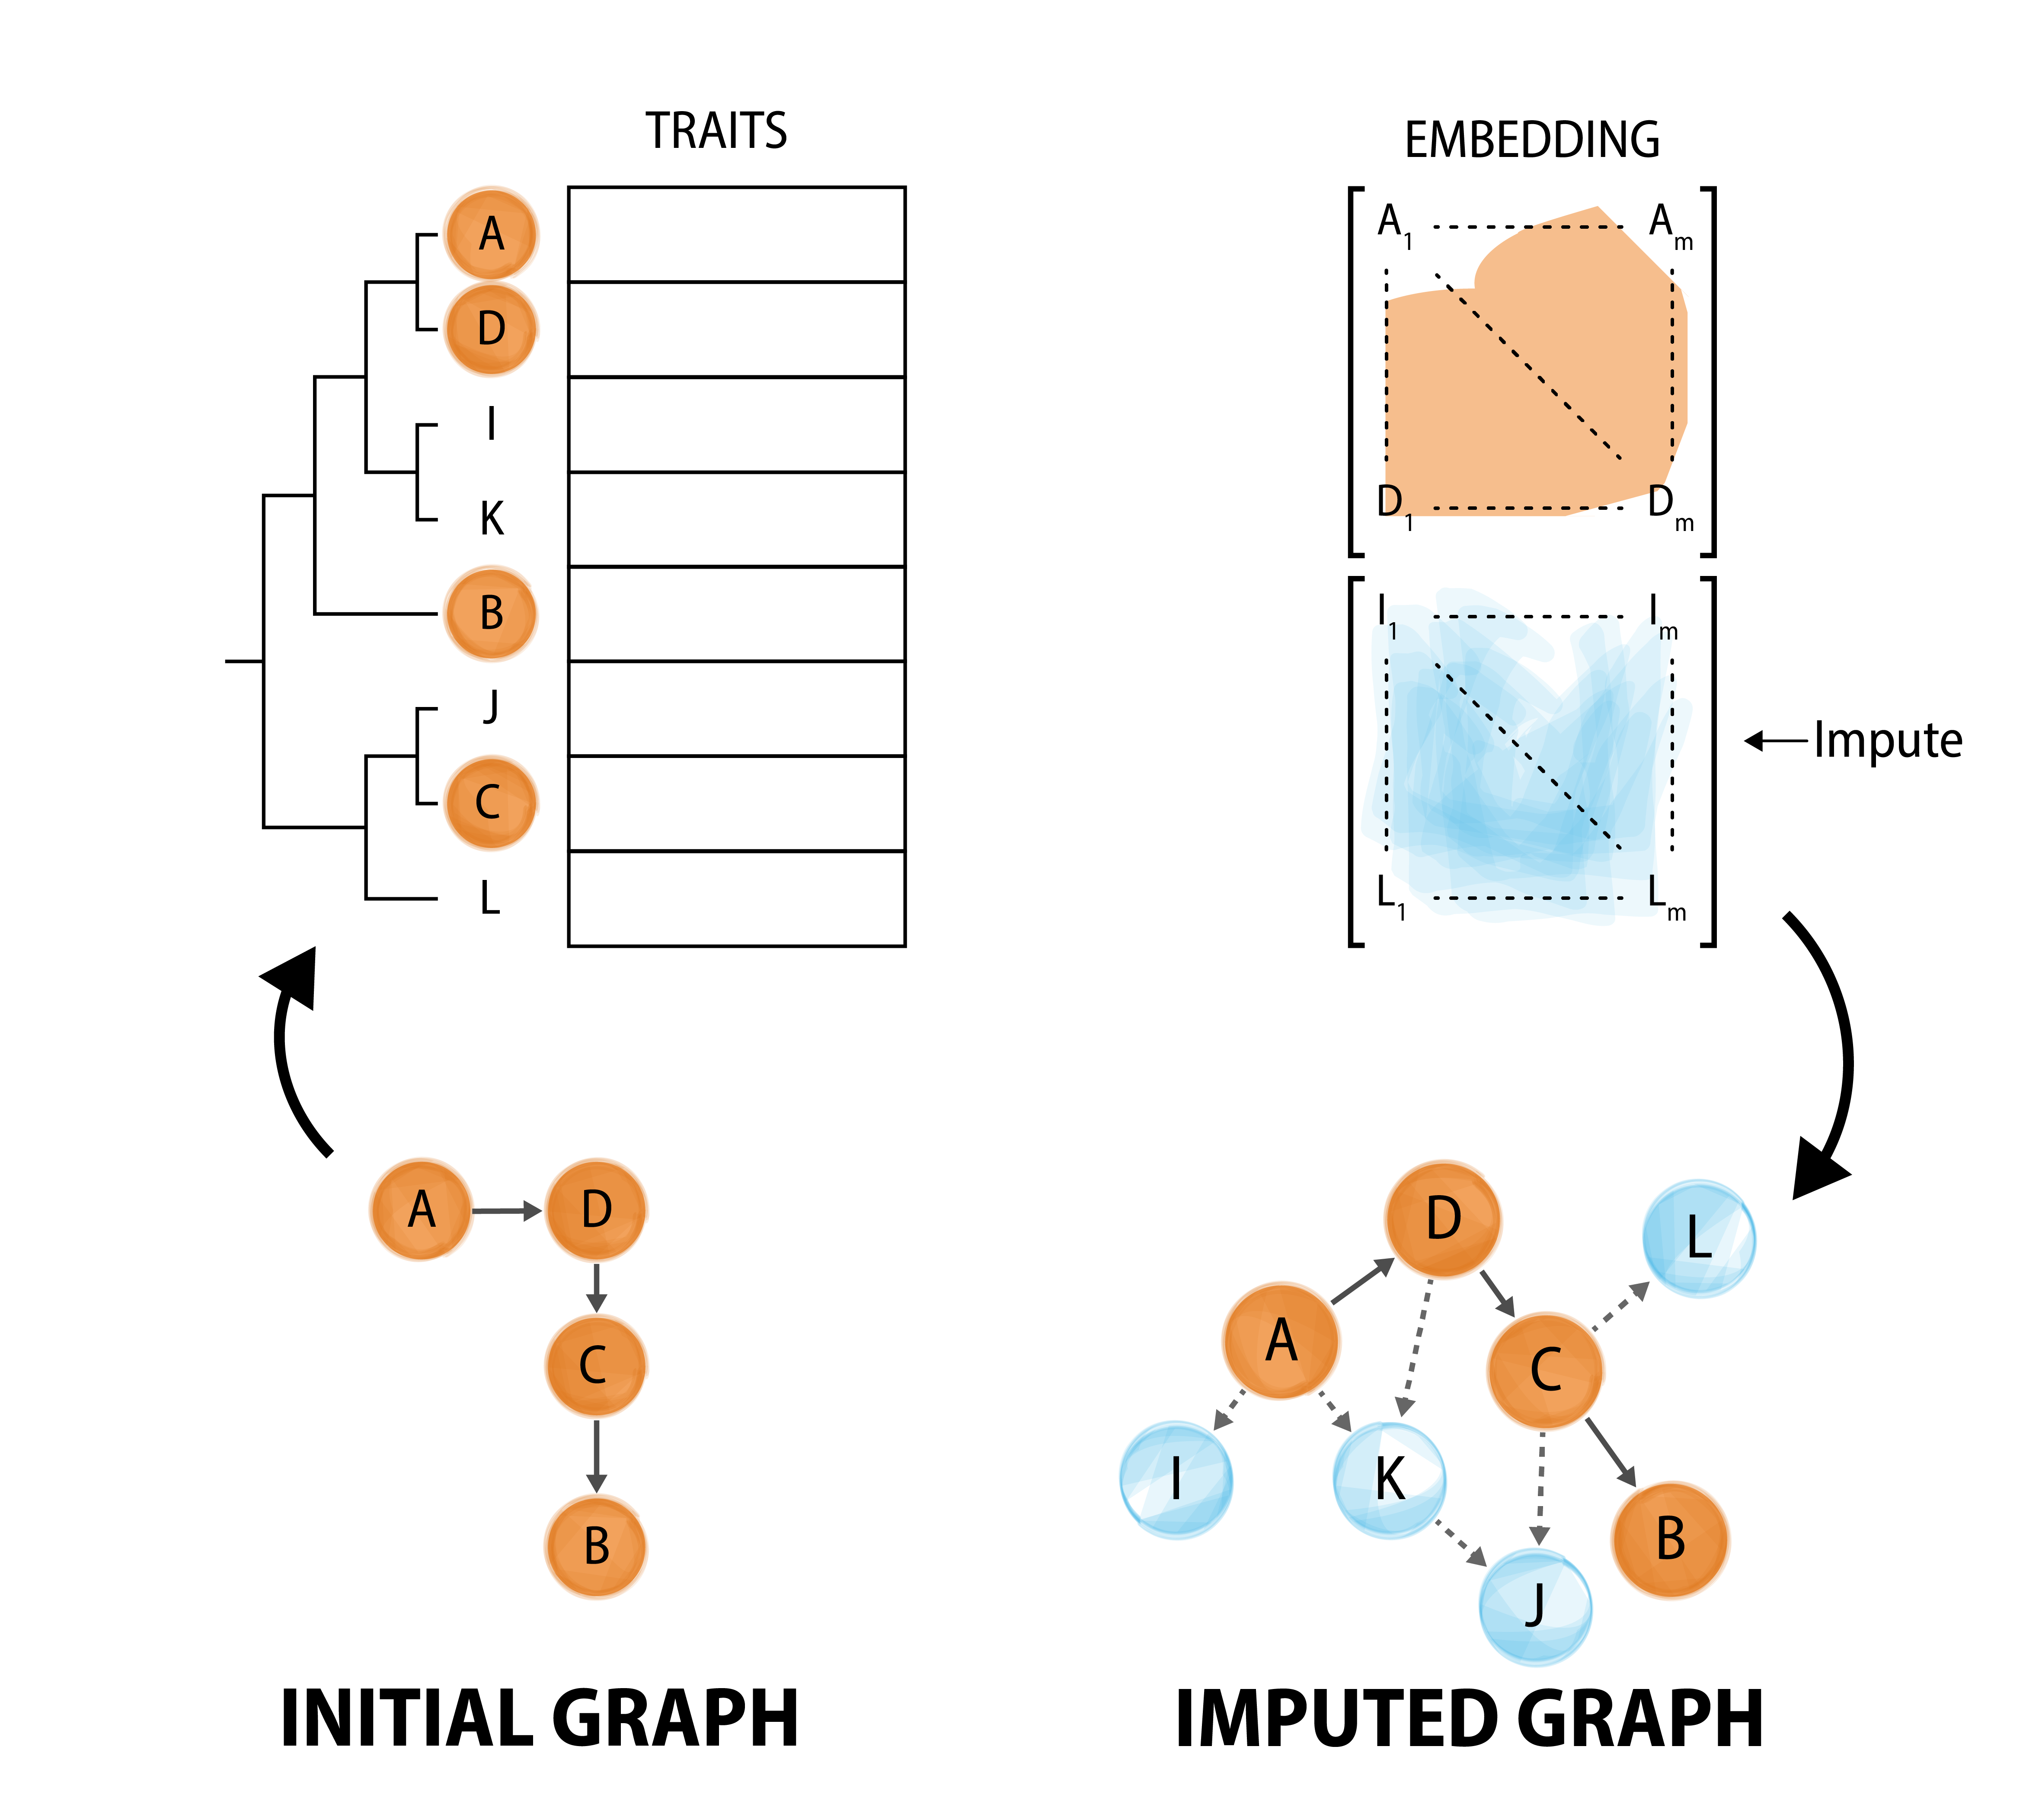
\includegraphics{figures/conceptual_prediction.png}
\caption{From a low-dimensional feature vector (see
fig.~\ref{fig:embedding}), it is possible to develop predictive
approaches. Nodes in an ecological network are species, for which we can
leverage phylogenetic relatedness (\emph{e.g.} Strydom, Bouskila, et
al., 2021) or functional traits to fill the values of additional species
we would like to project in this space (here, I, J, K, and L) from the
embedding of known species (here, A, B, C, and D). Because embeddings
can be projected back to a graph, this allows us to reconstruct a
network with these new species. This approach constitutes an instance of
transfer learning.}\label{fig:prediction}
}
\end{figure}

\hypertarget{the-metaweb-embeds-ecological-hypotheses-and-practices}{%
\section{The metaweb embeds ecological hypotheses and
practices}\label{the-metaweb-embeds-ecological-hypotheses-and-practices}}

The goal of metaweb inference is to provide information about the
interactions between species at a large spatial scale. But as Herbert
(1965) rightfully pointed out, ``{[}y{]}ou can't draw neat lines around
planet-wide problems''; any inference of a metaweb at large scales must
contend with several novel, and interwoven, families of problems.

The first is the taxonomic and spatial limit of the metaweb to embed and
transfer. If the initial metaweb is too narrow in scope, notably from a
taxonomic point of view, the chances of finding another area with enough
related species (through phylogenetic relatedness or similarity of
functional traits) to make a reliable inference decreases; this would
likely be indicated by large confidence intervals during estimation of
the values in the low-rank space, or by non-overlapping trait
distributions in the known and unknown species. Alternatively a metaweb
is too large (taxonomically), then the resulting embeddings would have
interactions relative to taxonomic groups that not present in the new
location, resulting in the potential under or over estimation of the
strength of new predicted interactions. The lack of well documented
metawebs is currently preventing the development of more concrete
guidelines. The question of phylogenetic relatedness and dispersal is
notably true if the metaweb is assembled in an area with mostly endemic
species (\emph{e.g.} a system that has undergone recent radiation and
might not have an analogous system with which to draw knowledge from),
and as with every predictive algorithm, there is room for the
application of our best ecological judgement.

The second series of problems relate to determining which area should be
used to infer the new metaweb in, as this determines the species pool
that must be used. Metawebs can be constructed by assigning interactions
in a list of species within geographic boundaries. The upside of this
approach is that information at the country level is likely to be
required for biodiversity assessments, as countries set goals at the
national level (Buxton et al., 2021), and as quantitative instruments
are designed to work at these scales (Turak et al., 2017); specific
strategies are often enacted at smaller scales, nested within a specific
country (Ray et al., 2021). But there is no guarantee that these
boundaries are meaningful. In fact, we do not have a satisfying answer
to the question of ``where does a food web stop?''; the most promising
solutions involve examining the spatial consistency of network area
relationships (Fortin et al., 2021; see \emph{e.g.} Galiana et al.,
2018, 2019, 2021), which is impossible in the absence of enough
information about the network itself. This suggests that inferred
metawebs should be further downscaled to allow for \emph{a posteriori}
analyses.

The final family of problems relates less to ecological concepts and
more to the praxis of ecological research. Operating under the context
of national divisions, in large parts of the world, reflects nothing
more than the legacy of settler colonialism, which not only drive a
disparity in available ecological data, but can entrench said biases
with the machine learning models that make predictions with them.
Indeed, the use of ecological data is not an apolitical act (Nost \&
Goldstein, 2021), as data infrastructures tend to be designed to answer
questions within national boundaries, and their use often draws upon and
reinforces territorial statecraft. As per Machen \& Nost (2021), this is
particularly true when the output of ``algorithmic thinking''
(\emph{e.g.} relying on machine learning to generate knowledge) can be
re-used for governance (\emph{e.g.} enacting conservation decisions at
the national scale). We therefore recognize that predictive approaches
deployed at the continental scale, no matter their intent, originate in
the framework that contributed to the ongoing biodiversity crisis (Adam,
2014), reinforced environmental injustice (Choudry, 2013; Domínguez \&
Luoma, 2020), and \emph{e.g.} as on Turtle Island, should be replaced by
Indigenous principles of land management (Eichhorn et al., 2019; No'kmaq
et al., 2021). As we see artificial intelligence/machine learning being
increasingly mobilized to generate knowledge that is lacking for
conservation decisions (\emph{e.g.} Lamba et al., 2019; Mosebo Fernandes
et al., 2020) and drive policy decisions (Weiskopf et al., 2022), our
discussion of these tools need to go beyond the technical, and into the
governance consequences they can have.

\textbf{Acknowledgements:} We acknowledge that this study was conducted
on land within the traditional unceded territory of the Saint Lawrence
Iroquoian, Anishinabewaki, Mohawk, Huron-Wendat, and Omàmiwininiwak
nations. TP, TS, DC, and LP received funding from the Canadian Institute
for Ecology \& Evolution. FB is funded by the Institute for Data
Valorization (IVADO). TS, SB, and TP are funded by a donation from the
Courtois Foundation. CB was awarded a Mitacs Elevate Fellowship no.
IT12391, in partnership with fRI Research, and also acknowledges funding
from Alberta Innovates and the Forest Resources Improvement Association
of Alberta. M-JF acknowledges funding from NSERC Discovery Grant and
NSERC CRC. RR is funded by New Zealand's Biological Heritage Ngā Koiora
Tuku Iho National Science Challenge, administered by New Zealand
Ministry of Business, Innovation, and Employment. BM is funded by the
NSERC Alexander Graham Bell Canada Graduate Scholarship and the FRQNT
master's scholarship. LP acknowledges funding from NSERC Discovery Grant
(NSERC RGPIN-2019-05771). TP acknowledges financial support from NSERC
through the Discovery Grants and Discovery Accelerator Supplement
programs. MJF is supported by an NSERC PDF and an RBC Post-Doctoral
Fellowship

\textbf{Conflict of interest:} The authors have no conflict interests to
disclose

\textbf{Authors' contributions:} TS, and TP conceived the ideas
discussed in the manuscript. All authors contributed to writing and
editing the manuscript.

\textbf{Data availability:} There is no data associated with this
manuscript.

\hypertarget{references}{%
\section*{References}\label{references}}
\addcontentsline{toc}{section}{References}

\hypertarget{refs}{}
\begin{CSLReferences}{1}{0}
\leavevmode\hypertarget{ref-Adam2014EleTre}{}%
Adam, R. (2014). \emph{Elephant treaties: The Colonial legacy of the
biodiversity crisis}. UPNE.

\leavevmode\hypertarget{ref-Albouy2019MarFis}{}%
Albouy, C., Archambault, P., Appeltans, W., Araújo, M. B., Beauchesne,
D., Cazelles, K., Cirtwill, A. R., Fortin, M.-J., Galiana, N., Leroux,
S. J., Pellissier, L., Poisot, T., Stouffer, D. B., Wood, S. A., \&
Gravel, D. (2019). The marine fish food web is globally connected.
\emph{Nature Ecology \& Evolution}, \emph{3}(8, 8), 1153--1161.
\url{https://doi.org/10.1038/s41559-019-0950-y}

\leavevmode\hypertarget{ref-Arsov2019NetEmb}{}%
Arsov, N., \& Mirceva, G. (2019, November 26). \emph{Network Embedding:
An Overview}. \url{http://arxiv.org/abs/1911.11726}

\leavevmode\hypertarget{ref-Bartomeus2016ComFra}{}%
Bartomeus, I., Gravel, D., Tylianakis, J. M., Aizen, M. A., Dickie, I.
A., \& Bernard-Verdier, M. (2016). A common framework for identifying
linkage rules across different types of interactions. \emph{Functional
Ecology}, \emph{30}(12), 1894--1903.

\leavevmode\hypertarget{ref-Botella2022AppGra}{}%
Botella, C., Dray, S., Matias, C., Miele, V., \& Thuiller, W. (2022). An
appraisal of graph embeddings for comparing trophic network
architectures. \emph{Methods in Ecology and Evolution}, \emph{13}(1),
203--216. \url{https://doi.org/10.1111/2041-210X.13738}

\leavevmode\hypertarget{ref-Braga2019SpaAna}{}%
Braga, J., Pollock, L. J., Barros, C., Galiana, N., Montoya, J. M.,
Gravel, D., Maiorano, L., Montemaggiori, A., Ficetola, G. F., Dray, S.,
\& Thuiller, W. (2019). Spatial analyses of multi-trophic terrestrial
vertebrate assemblages in Europe. \emph{Global Ecology and
Biogeography}, \emph{28}(11), 1636--1648.
\url{https://doi.org/10.1111/geb.12981}

\leavevmode\hypertarget{ref-BramonMora2018IdeCom}{}%
Bramon Mora, B., Gravel, D., Gilarranz, L. J., Poisot, T., \& Stouffer,
D. B. (2018). Identifying a common backbone of interactions underlying
food webs from different ecosystems. \emph{Nature Communications},
\emph{9}(1), 2603. \url{https://doi.org/10.1038/s41467-018-05056-0}

\leavevmode\hypertarget{ref-Buxton2021KeyInf}{}%
Buxton, R. T., Bennett, J. R., Reid, A. J., Shulman, C., Cooke, S. J.,
Francis, C. M., Nyboer, E. A., Pritchard, G., Binley, A. D., Avery-Gomm,
S., Ban, N. C., Beazley, K. F., Bennett, E., Blight, L. K., Bortolotti,
L. E., Camfield, A. F., Gadallah, F., Jacob, A. L., Naujokaitis-Lewis,
I., \ldots{} Smith, P. A. (2021). Key information needs to move from
knowledge to action for biodiversity conservation in Canada.
\emph{Biological Conservation}, \emph{256}, 108983.
\url{https://doi.org/10.1016/j.biocon.2021.108983}

\leavevmode\hypertarget{ref-Chen2017DeeMul}{}%
Chen, D., Xue, Y., Fink, D., Chen, S., \& Gomes, C. P. (2017).
\emph{Deep Multi-species Embedding}. 3639--3646.

\leavevmode\hypertarget{ref-Chen2017HarHie}{}%
Chen, H., Perozzi, B., Hu, Y., \& Skiena, S. (2017, November 16).
\emph{HARP: Hierarchical Representation Learning for Networks}.
\url{http://arxiv.org/abs/1706.07845}

\leavevmode\hypertarget{ref-Choudry2013SavBio}{}%
Choudry, A. (2013). Saving biodiversity, for whom and for what?
Conservation NGOs, complicity, colonialism and conquest in an era of
capitalist globalization. In \emph{NGOization: Complicity,
contradictions and prospects} (pp. 24--44). Bloomsbury Publishing.

\leavevmode\hypertarget{ref-Cieslak2020TdiSto}{}%
Cieslak, M. C., Castelfranco, A. M., Roncalli, V., Lenz, P. H., \&
Hartline, D. K. (2020). T-Distributed Stochastic Neighbor Embedding
(t-SNE): A tool for eco-physiological transcriptomic analysis.
\emph{Marine Genomics}, \emph{51}, 100723.
\url{https://doi.org/10.1016/j.margen.2019.100723}

\leavevmode\hypertarget{ref-Csermely2004StrLin}{}%
Csermely, P. (2004). Strong links are important, but weak links
stabilize them. \emph{Trends in Biochemical Sciences}, \emph{29}(7),
331--334. \url{https://doi.org/10.1016/j.tibs.2004.05.004}

\leavevmode\hypertarget{ref-DallaRiva2016ExpEvo}{}%
Dalla Riva, G. V., \& Stouffer, D. B. (2016). Exploring the evolutionary
signature of food webs' backbones using functional traits. \emph{Oikos},
\emph{125}(4), 446--456. \url{https://doi.org/10.1111/oik.02305}

\leavevmode\hypertarget{ref-Dallas2017PreCry}{}%
Dallas, T., Park, A. W., \& Drake, J. M. (2017). Predicting cryptic
links in host-parasite networks. \emph{PLOS Computational Biology},
\emph{13}(5), e1005557.
\url{https://doi.org/10.1371/journal.pcbi.1005557}

\leavevmode\hypertarget{ref-Dominguez2020DecCon}{}%
Domínguez, L., \& Luoma, C. (2020). Decolonising Conservation Policy:
How Colonial Land and Conservation Ideologies Persist and Perpetuate
Indigenous Injustices at the Expense of the Environment. \emph{Land},
\emph{9}(3, 3), 65. \url{https://doi.org/10.3390/land9030065}

\leavevmode\hypertarget{ref-Dunne2006NetStr}{}%
Dunne, J. A. (2006). The Network Structure of Food Webs. In J. A. Dunne
\& M. Pascual (Eds.), \emph{Ecological networks: Linking structure and
dynamics} (pp. 27--86). Oxford University Press.

\leavevmode\hypertarget{ref-Eichhorn2019SteDec}{}%
Eichhorn, M. P., Baker, K., \& Griffiths, M. (2019). Steps towards
decolonising biogeography. \emph{Frontiers of Biogeography},
\emph{12}(1), 1--7. \url{https://doi.org/10.21425/F5FBG44795}

\leavevmode\hypertarget{ref-Eklof2013DimEco}{}%
Eklöf, A., Jacob, U., Kopp, J., Bosch, J., Castro-Urgal, R., Chacoff, N.
P., Dalsgaard, B., de Sassi, C., Galetti, M., Guimarães, P. R.,
Lomáscolo, S. B., Martín González, A. M., Pizo, M. A., Rader, R.,
Rodrigo, A., Tylianakis, J. M., Vázquez, D. P., \& Allesina, S. (2013).
The dimensionality of ecological networks. \emph{Ecology Letters},
\emph{16}(5), 577--583. \url{https://doi.org/10.1111/ele.12081}

\leavevmode\hypertarget{ref-Fortin2021NetEco}{}%
Fortin, M.-J., Dale, M. R. T., \& Brimacombe, C. (2021). Network ecology
in dynamic landscapes. \emph{Proceedings of the Royal Society B:
Biological Sciences}, \emph{288}(1949), rspb.2020.1889, 20201889.
\url{https://doi.org/10.1098/rspb.2020.1889}

\leavevmode\hypertarget{ref-Fricke2022EffDef}{}%
Fricke, E. C., Ordonez, A., Rogers, H. S., \& Svenning, J.-C. (2022).
The effects of defaunation on plants' capacity to track climate change.
\emph{Science}.

\leavevmode\hypertarget{ref-Galiana2021SpaSca}{}%
Galiana, N., Barros, C., Braga, J., Ficetola, G. F., Maiorano, L.,
Thuiller, W., Montoya, J. M., \& Lurgi, M. (2021). The spatial scaling
of food web structure across European biogeographical regions.
\emph{Ecography}, \emph{n/a}(n/a).
\url{https://doi.org/10.1111/ecog.05229}

\leavevmode\hypertarget{ref-Galiana2019GeoVar}{}%
Galiana, N., Hawkins, B. A., \& Montoya, J. M. (2019). The geographical
variation of network structure is scale dependent: Understanding the
biotic specialization of hostparasitoid networks. \emph{Ecography},
\emph{42}(6), 1175--1187. \url{https://doi.org/10.1111/ecog.03684}

\leavevmode\hypertarget{ref-Galiana2022EcoNet}{}%
Galiana, N., Lurgi, M., Bastazini, V. A. G., Bosch, J., Cagnolo, L.,
Cazelles, K., Claramunt-López, B., Emer, C., Fortin, M.-J., Grass, I.,
Hernández-Castellano, C., Jauker, F., Leroux, S. J., McCann, K., McLeod,
A. M., Montoya, D., Mulder, C., Osorio-Canadas, S., Reverté, S.,
\ldots{} Montoya, J. M. (2022). Ecological network complexity scales
with area. \emph{Nature Ecology \& Evolution}, 1--8.
\url{https://doi.org/10.1038/s41559-021-01644-4}

\leavevmode\hypertarget{ref-Galiana2018SpaSca}{}%
Galiana, N., Lurgi, M., Claramunt-López, B., Fortin, M.-J., Leroux, S.,
Cazelles, K., Gravel, D., \& Montoya, J. M. (2018). The spatial scaling
of species interaction networks. \emph{Nature Ecology \& Evolution},
\emph{2}(5), 782--790. \url{https://doi.org/10.1038/s41559-018-0517-3}

\leavevmode\hypertarget{ref-Goyal2018GraEmb}{}%
Goyal, P., \& Ferrara, E. (2018). Graph embedding techniques,
applications, and performance: A survey. \emph{Knowledge-Based Systems},
\emph{151}, 78--94. \url{https://doi.org/10.1016/j.knosys.2018.03.022}

\leavevmode\hypertarget{ref-Gravel2018BriElt}{}%
Gravel, D., Baiser, B., Dunne, J. A., Kopelke, J.-P., Martinez, N. D.,
Nyman, T., Poisot, T., Stouffer, D. B., Tylianakis, J. M., Wood, S. A.,
\& Roslin, T. (2018). Bringing Elton and Grinnell together: A
quantitative framework to represent the biogeography of ecological
interaction networks. \emph{Ecography}, \emph{0}(0).
\url{https://doi.org/10.1111/ecog.04006}

\leavevmode\hypertarget{ref-Grover2016NodSca}{}%
Grover, A., \& Leskovec, J. (2016). Node2vec: Scalable Feature Learning
for Networks. \emph{Proceedings of the 22nd ACM SIGKDD International
Conference on Knowledge Discovery and Data Mining}, 855--864.
\url{https://doi.org/10.1145/2939672.2939754}

\leavevmode\hypertarget{ref-Grunig2020CroFor}{}%
Grünig, M., Mazzi, D., Calanca, P., Karger, D. N., \& Pellissier, L.
(2020). Crop and forest pest metawebs shift towards increased linkage
and suitability overlap under climate change. \emph{Communications
Biology}, \emph{3}(1, 1), 1--10.
\url{https://doi.org/10.1038/s42003-020-0962-9}

\leavevmode\hypertarget{ref-Herbert1965Dun}{}%
Herbert, F. (1965). \emph{Dune} (1st ed.). Chilton Book Company.

\leavevmode\hypertarget{ref-Hinton2002StoNei}{}%
Hinton, G., \& Roweis, S. T. (2002). Stochastic neighbor embedding.
\emph{NIPS}, \emph{15}, 833--840.

\leavevmode\hypertarget{ref-Hoffmann2019MacLea}{}%
Hoffmann, J., Bar-Sinai, Y., Lee, L. M., Andrejevic, J., Mishra, S.,
Rubinstein, S. M., \& Rycroft, C. H. (2019). Machine learning in a
data-limited regime: Augmenting experiments with synthetic data uncovers
order in crumpled sheets. \emph{Science Advances}, \emph{5}(4),
eaau6792. \url{https://doi.org/10.1126/sciadv.aau6792}

\leavevmode\hypertarget{ref-Hortal2015SevSho}{}%
Hortal, J., de Bello, F., Diniz-Filho, J. A. F., Lewinsohn, T. M., Lobo,
J. M., \& Ladle, R. J. (2015). Seven Shortfalls that Beset Large-Scale
Knowledge of Biodiversity. \emph{Annual Review of Ecology, Evolution,
and Systematics}, \emph{46}(1), 523--549.
\url{https://doi.org/10.1146/annurev-ecolsys-112414-054400}

\leavevmode\hypertarget{ref-Jordano2016SamNet}{}%
Jordano, P. (2016). Sampling networks of ecological interactions.
\emph{Functional Ecology}, \emph{30}(12), 1883--1893.
\url{https://doi.org/10.1111/1365-2435.12763}

\leavevmode\hypertarget{ref-Lamba2019DeeLea}{}%
Lamba, A., Cassey, P., Segaran, R. R., \& Koh, L. P. (2019). Deep
learning for environmental conservation. \emph{Current Biology},
\emph{29}(19), R977--R982.
\url{https://doi.org/10.1016/j.cub.2019.08.016}

\leavevmode\hypertarget{ref-Machen2021ThiAlg}{}%
Machen, R., \& Nost, E. (2021). Thinking algorithmically: The making of
hegemonic knowledge in climate governance. \emph{Transactions of the
Institute of British Geographers}, \emph{46}(3), 555--569.
\url{https://doi.org/10.1111/tran.12441}

\leavevmode\hypertarget{ref-McLeod2021SamAsy}{}%
McLeod, A., Leroux, S. J., Gravel, D., Chu, C., Cirtwill, A. R., Fortin,
M.-J., Galiana, N., Poisot, T., \& Wood, S. A. (2021). Sampling and
asymptotic network properties of spatial multi-trophic networks.
\emph{Oikos}, \emph{n/a}(n/a). \url{https://doi.org/10.1111/oik.08650}

\leavevmode\hypertarget{ref-Melnyk2020GraGra}{}%
Melnyk, K., Klus, S., Montavon, G., \& Conrad, T. O. F. (2020).
GraphKKE: Graph Kernel Koopman embedding for human microbiome analysis.
\emph{Applied Network Science}, \emph{5}(1), 96.
\url{https://doi.org/10.1007/s41109-020-00339-2}

\leavevmode\hypertarget{ref-Morales-Castilla2015InfBio}{}%
Morales-Castilla, I., Matias, M. G., Gravel, D., \& Araújo, M. B.
(2015). Inferring biotic interactions from proxies. \emph{Trends in
Ecology \& Evolution}, \emph{30}(6), 347--356.
\url{https://doi.org/10.1016/j.tree.2015.03.014}

\leavevmode\hypertarget{ref-MoseboFernandes2020MacLea}{}%
Mosebo Fernandes, A. C., Quintero Gonzalez, R., Lenihan-Clarke, M. A.,
Leslie Trotter, E. F., \& Jokar Arsanjani, J. (2020). Machine Learning
for Conservation Planning in a Changing Climate. \emph{Sustainability},
\emph{12}(18, 18), 7657. \url{https://doi.org/10.3390/su12187657}

\leavevmode\hypertarget{ref-Murphy2022ProMac}{}%
Murphy, K. P. (2022). \emph{Probabilistic machine learning: An
introduction}. MIT Press.

\leavevmode\hypertarget{ref-Narayanan2017GraLea}{}%
Narayanan, A., Chandramohan, M., Venkatesan, R., Chen, L., Liu, Y., \&
Jaiswal, S. (2017, July 17). \emph{Graph2vec: Learning Distributed
Representations of Graphs}. \url{http://arxiv.org/abs/1707.05005}

\leavevmode\hypertarget{ref-Neutel2002StaRea}{}%
Neutel, A.-M., Heesterbeek, J. A. P., \& de Ruiter, P. C. (2002).
Stability in Real Food Webs: Weak Links in Long Loops. \emph{Science},
\emph{296}(5570), 1120--1123.
\url{https://doi.org/10.1126/science.1068326}

\leavevmode\hypertarget{ref-Nokmaq2021AwaSle}{}%
No'kmaq, M., Marshall, A., Beazley, K. F., Hum, J., joudry, shalan,
Papadopoulos, A., Pictou, S., Rabesca, J., Young, L., \& Zurba, M.
(2021). {``Awakening the sleeping giant''}: Re-Indigenization principles
for transforming biodiversity conservation in Canada and beyond.
\emph{FACETS}, \emph{6}(1), 839--869.

\leavevmode\hypertarget{ref-Nost2021PolEco}{}%
Nost, E., \& Goldstein, J. E. (2021). A political ecology of data.
\emph{Environment and Planning E: Nature and Space}, 25148486211043503.
\url{https://doi.org/10.1177/25148486211043503}

\leavevmode\hypertarget{ref-OConnor2020UnvFoo}{}%
O'Connor, L. M. J., Pollock, L. J., Braga, J., Ficetola, G. F.,
Maiorano, L., Martinez-Almoyna, C., Montemaggiori, A., Ohlmann, M., \&
Thuiller, W. (2020). Unveiling the food webs of tetrapods across Europe
through the prism of the Eltonian niche. \emph{Journal of Biogeography},
\emph{47}(1), 181--192. \url{https://doi.org/10.1111/jbi.13773}

\leavevmode\hypertarget{ref-Pedersen2017SigCol}{}%
Pedersen, E. J., Thompson, P. L., Ball, R. A., Fortin, M.-J., Gouhier,
T. C., Link, H., Moritz, C., Nenzen, H., Stanley, R. R. E., Taranu, Z.
E., Gonzalez, A., Guichard, F., \& Pepin, P. (2017). Signatures of the
collapse and incipient recovery of an overexploited marine ecosystem.
\emph{Royal Society Open Science}, \emph{4}(7), 170215.
\url{https://doi.org/10.1098/rsos.170215}

\leavevmode\hypertarget{ref-Perozzi2014DeeOnl}{}%
Perozzi, B., Al-Rfou, R., \& Skiena, S. (2014). DeepWalk: Online
learning of social representations. \emph{Proceedings of the 20th ACM
SIGKDD International Conference on Knowledge Discovery and Data Mining},
701--710. \url{https://doi.org/10.1145/2623330.2623732}

\leavevmode\hypertarget{ref-Pichler2020MacLea}{}%
Pichler, M., Boreux, V., Klein, A.-M., Schleuning, M., \& Hartig, F.
(2020). Machine learning algorithms to infer trait-matching and predict
species interactions in ecological networks. \emph{Methods in Ecology
and Evolution}, \emph{11}(2), 281--293.
\url{https://doi.org/10.1111/2041-210X.13329}

\leavevmode\hypertarget{ref-Poisot2016StrPro}{}%
Poisot, T., Cirtwill, A. R., Cazelles, K., Gravel, D., Fortin, M.-J., \&
Stouffer, D. B. (2016). The structure of probabilistic networks.
\emph{Methods in Ecology and Evolution}, \emph{7}(3), 303--312.
\url{https://doi.org/10.1111/2041-210X.12468}

\leavevmode\hypertarget{ref-Poisot2021ImpMam}{}%
Poisot, T., Ouellet, M.-A., Mollentze, N., Farrell, M. J., Becker, D.
J., Albery, G. F., Gibb, R. J., Seifert, S. N., \& Carlson, C. J. (2021,
May 31). \emph{Imputing the mammalian virome with linear filtering and
singular value decomposition}. \url{http://arxiv.org/abs/2105.14973}

\leavevmode\hypertarget{ref-Poisot2015SpeWhy}{}%
Poisot, T., Stouffer, D. B., \& Gravel, D. (2015). Beyond species: Why
ecological interaction networks vary through space and time.
\emph{Oikos}, \emph{124}(3), 243--251.
\url{https://doi.org/10.1111/oik.01719}

\leavevmode\hypertarget{ref-Ramasamy2015ComSpe}{}%
Ramasamy, D., \& Madhow, U. (2015). Compressive spectral embedding:
Sidestepping the SVD. In C. Cortes, N. Lawrence, D. Lee, M. Sugiyama, \&
R. Garnett (Eds.), \emph{Advances in neural information processing
systems} (Vol. 28). Curran Associates, Inc.

\leavevmode\hypertarget{ref-Ray2021BioCri}{}%
Ray, J. C., Grimm, J., \& Olive, A. (2021). The biodiversity crisis in
Canada: Failures and challenges of federal and sub-national strategic
and legal frameworks. \emph{FACETS}, \emph{6}, 1044--1068.
\url{https://doi.org/10.1139/facets-2020-0075}

\leavevmode\hypertarget{ref-Runghen2021ExpNod}{}%
Runghen, R., Stouffer, D. B., \& Dalla Riva, G. V. (2021).
\emph{Exploiting node metadata to predict interactions in large networks
using graph embedding and neural networks}.
\url{https://doi.org/10.1101/2021.06.10.447991}

\leavevmode\hypertarget{ref-Saravia2021EcoNet}{}%
Saravia, L. A., Marina, T. I., Kristensen, N. P., De Troch, M., \& Momo,
F. R. (2021). Ecological network assembly: How the regional metaweb
influences local food webs. \emph{Journal of Animal Ecology},
\emph{n/a}(n/a). \url{https://doi.org/10.1111/1365-2656.13652}

\leavevmode\hypertarget{ref-Strydom2021FooWeb}{}%
Strydom, T., Bouskila, S., Banville, F., Barros, C., Caron, D., Farrell,
M. J., Fortin, M.-J., Hemming, V., Mercier, B., Pollock, L., Runghen,
R., Riva, G. V. D., \& Poisot, T. (2021). \emph{Food web reconstruction
through phylogenetic transfer of low-rank network representation}.
\url{https://doi.org/10.32942/osf.io/y7sdz}

\leavevmode\hypertarget{ref-Strydom2021RoaPre}{}%
Strydom, T., Catchen, M. D., Banville, F., Caron, D., Dansereau, G.,
Desjardins-Proulx, P., Forero-Muñoz, N. R., Higino, G., Mercier, B.,
Gonzalez, A., Gravel, D., Pollock, L., \& Poisot, T. (2021). A roadmap
towards predicting species interaction networks (across space and time).
\emph{Philosophical Transactions of the Royal Society B: Biological
Sciences}, \emph{376}(1837), 20210063.
\url{https://doi.org/10.1098/rstb.2021.0063}

\leavevmode\hypertarget{ref-Tang2015LinLar}{}%
Tang, J., Qu, M., Wang, M., Zhang, M., Yan, J., \& Mei, Q. (2015). LINE:
Large-scale Information Network Embedding. \emph{Proceedings of the 24th
International Conference on World Wide Web}, 1067--1077.
\url{https://doi.org/10.1145/2736277.2741093}

\leavevmode\hypertarget{ref-Turak2017UsiEss}{}%
Turak, E., Brazill-Boast, J., Cooney, T., Drielsma, M., DelaCruz, J.,
Dunkerley, G., Fernandez, M., Ferrier, S., Gill, M., Jones, H., Koen,
T., Leys, J., McGeoch, M., Mihoub, J.-B., Scanes, P., Schmeller, D., \&
Williams, K. (2017). Using the essential biodiversity variables
framework to measure biodiversity change at national scale.
\emph{Biological Conservation}, \emph{213}, 264--271.
\url{https://doi.org/10.1016/j.biocon.2016.08.019}

\leavevmode\hypertarget{ref-Wang2016StrDee}{}%
Wang, D., Cui, P., \& Zhu, W. (2016). Structural Deep Network Embedding.
\emph{Proceedings of the 22nd ACM SIGKDD International Conference on
Knowledge Discovery and Data Mining}, 1225--1234.
\url{https://doi.org/10.1145/2939672.2939753}

\leavevmode\hypertarget{ref-Wang2021JoiEmb}{}%
Wang, S., Arroyo, J., Vogelstein, J. T., \& Priebe, C. E. (2021). Joint
Embedding of Graphs. \emph{IEEE Transactions on Pattern Analysis and
Machine Intelligence}, \emph{43}(4), 1324--1336.
\url{https://doi.org/10.1109/TPAMI.2019.2948619}

\leavevmode\hypertarget{ref-Wardeh2021PreMam}{}%
Wardeh, M., Baylis, M., \& Blagrove, M. S. C. (2021). Predicting
mammalian hosts in which novel coronaviruses can be generated.
\emph{Nature Communications}, \emph{12}(1, 1), 780.
\url{https://doi.org/10.1038/s41467-021-21034-5}

\leavevmode\hypertarget{ref-Weiskopf2022IncUpt}{}%
Weiskopf, S. R., Harmáčková, Z. V., Johnson, C. G., Londoño-Murcia, M.
C., Miller, B. W., Myers, B. J. E., Pereira, L., Arce-Plata, M. I.,
Blanchard, J. L., Ferrier, S., Fulton, E. A., Harfoot, M., Isbell, F.,
Johnson, J. A., Mori, A. S., Weng, E., \& Rosa, I. M. D. (2022).
Increasing the uptake of ecological model results in policy decisions to
improve biodiversity outcomes. \emph{Environmental Modelling \&
Software}, \emph{149}, 105318.
\url{https://doi.org/10.1016/j.envsoft.2022.105318}

\leavevmode\hypertarget{ref-Wood2015EffSpa}{}%
Wood, S. A., Russell, R., Hanson, D., Williams, R. J., \& Dunne, J. A.
(2015). Effects of spatial scale of sampling on food web structure.
\emph{Ecology and Evolution}, \emph{5}(17), 3769--3782.
\url{https://doi.org/10.1002/ece3.1640}

\leavevmode\hypertarget{ref-Xu2020UndGra}{}%
Xu, M. (2020, December 14). \emph{Understanding graph embedding methods
and their applications}. \url{http://arxiv.org/abs/2012.08019}

\leavevmode\hypertarget{ref-Yan2005GraEmb}{}%
Yan, S., Xu, D., Zhang, B., \& Zhang, H.-J. (2005). Graph embedding: A
general framework for dimensionality reduction. \emph{2005 IEEE Computer
Society Conference on Computer Vision and Pattern Recognition
(CVPR'05)}, \emph{2}, 830--837 vol. 2.
\url{https://doi.org/10.1109/CVPR.2005.170}

\leavevmode\hypertarget{ref-Young2007RanDot}{}%
Young, S. J., \& Scheinerman, E. R. (2007). Random Dot Product Graph
Models for Social Networks. In A. Bonato \& F. R. K. Chung (Eds.),
\emph{Algorithms and Models for the Web-Graph} (pp. 138--149). Springer.
\url{https://doi.org/10.1007/978-3-540-77004-6_11}

\end{CSLReferences}

\end{document}
